
%(BEGIN_QUESTION)
% Copyright 2006, Tony R. Kuphaldt, released under the Creative Commons Attribution License (v 1.0)
% This means you may do almost anything with this work of mine, so long as you give me proper credit

Qualitatively graph the response of a proportional-only controller over time to the following changes in process variable:

$$\includegraphics[width=15.5cm]{i01593x01.eps}$$

Assume {\it reverse} control action.

\vskip 20pt \vbox{\hrule \hbox{\strut \vrule{} {\bf Suggestions for Socratic discussion} \vrule} \hrule}

\begin{itemize}
\item{} What defines a ``reverse'' acting controller, in contrast to a ``direct'' acting controller?
\item{} Explain why it would be highly unusual to see a trend like this in a real, working process loop.  Why is this trend unrealistic, assuming a working process where all components are functioning properly?
\item{} Given that this trend is unrealistic, why is it something we're studying?  In other words, what value does a ``toy'' trend like this have for us?
\end{itemize}

\underbar{file i01593}
%(END_QUESTION)





%(BEGIN_ANSWER)

The controller output graph shown here is {\it qualitative} only.  Although drawn to scale (i.e. all changes in the output are properly scaled relative to each other), the scale itself is arbitrary and therefore may not match the scale of your sketch:

$$\includegraphics[width=15.5cm]{i01593x02.eps}$$

%(END_ANSWER)





%(BEGIN_NOTES)

Having a reverse control action means the output signal will move opposite that of the process variable.  I have drawn this graph for a proportional-only controller with a proportional band of 100\% (a gain of 1).

\vskip 10pt

{\bf Proportional control action is where the amount of error tells the output how \underbar{far} to go.}

\vskip 10pt

{\bf Integral control action is where the amount of error tells the output how \underbar{fast} to go.}

\vskip 10pt

{\bf Derivative control action is where \underbar{speed} of the error tells the output how \underbar{far} to go.}

%INDEX% Control, proportional: graphing controller response

%(END_NOTES)


